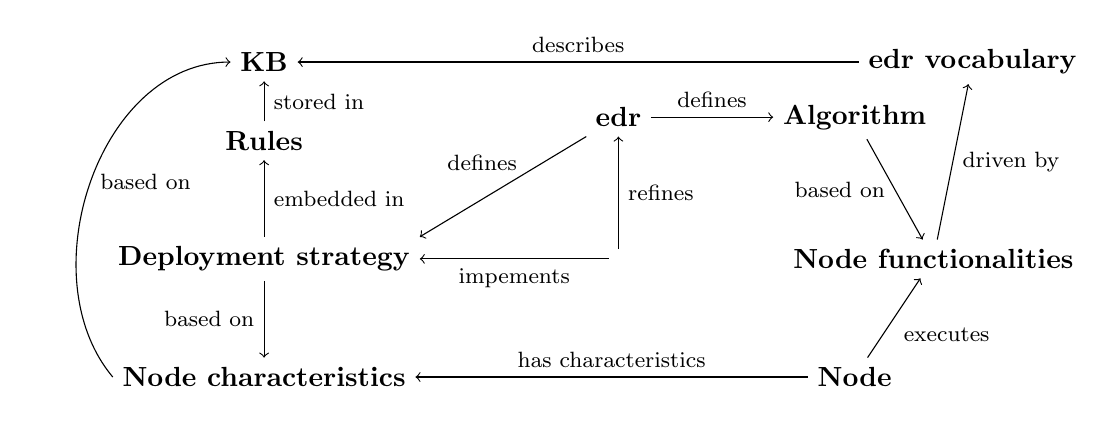
\begin{tikzpicture}
	\draw (-0.5,-1) node (characteristics) {\textbf{Node characteristics}};
	\draw (7, -1) node (node) {\textbf{Node}};
	\draw (-0.5, 0.5) node (strategy) {\textbf{Deployment strategy}};
	\draw (-0.5, 2) node (rules) {\textbf{Rules}};
	\draw (-0.5, 3) node (kb) {\textbf{KB}};
	\draw (4, 0.5) node (edrt) {\textbf{\edrt}};
	\draw (4, 2.3) node (edr) {\textbf{\gls{edr}}};
	\draw (7, 2.3) node (algorithm) {\textbf{Algorithm}};
	\draw (8, 0.5) node (functionalities) {\textbf{Node functionalities}};
	\draw (8.5 , 3) node (vocabulary) {\textbf{\gls{edr} vocabulary}};
	
	\draw[<-] (characteristics) -- node[above] {\footnotesize has characteristics} (node);
	\draw[->] (node) -- node[below right] {\footnotesize executes} (functionalities);
	\draw[->] (functionalities) -- node[right] {\footnotesize driven by} (vocabulary);
	\draw[->] (vocabulary) -- node[above] {\footnotesize describes} (kb);
	\draw[->] (rules) -- node[right] {\footnotesize stored in} (kb);
	\draw[->] (strategy) -- node[right] {\footnotesize embedded in} (rules);
	\draw[->] (edrt) -- node[below] {\footnotesize impements} (strategy);
	\draw[->] (edr) -- node[left, yshift=0.3cm, xshift=0.3cm] {\footnotesize defines} (strategy.north east);
	\draw[->] (edrt) -- node[right] {\footnotesize refines} (edr);
	\draw[->] (edr) -- node[above] {\footnotesize defines} (algorithm);
	\draw[->] (algorithm) -- node[left] {\footnotesize based on} (functionalities);
	\draw[->] (strategy) -- node[left] {\footnotesize based on} (characteristics);
	\draw[->] (characteristics.west) to[out=130, in=180] node[right] {\footnotesize based on} (kb.west);
	
\end{tikzpicture}